\documentclass[11pt,a4paper]{article}
\usepackage{bookmark}
\usepackage{graphicx,hyperref,amsmath,bm,url,amsthm}
\usepackage[table]{xcolor}
% \usepackage{fullpage}
\usepackage{lastpage}
\usepackage{enumitem}
\usepackage{fancyhdr}
%\usepackage{physics}
% \usepackage{mathrsfs}
\usepackage{mathtools}
\usepackage{wrapfig}
\usepackage{bm}
%\usepackage{fixdif}
\usepackage[square]{natbib}
\usepackage[utf8]{inputenc} % include umlaute

% -------- Define new color ------------------------------
\usepackage{color}  
\definecolor{darkblue}{rgb}{0.15,0,0.37}
\definecolor{darkred}{rgb}{0.35,0,0.08}
\definecolor{mygrey}{rgb}{0.85,0.85,0.85} % make grey for the table
% --------------------------------------------------------

\hypersetup{
colorlinks=true,
hypertexnames=false,
colorlinks,		
linkcolor={blue},
citecolor={blue},
urlcolor={blue},
%ocgcolorlinks, % this option changes the link color to black when the document is printed, for legibility in b/w 
pdfstartview={FitV},
unicode,
breaklinks=true
} 

\usepackage{microtype,todonotes}
\usepackage[australian]{babel} % change date to to European format
\usepackage[a4paper,text={14.5cm, 25.2cm},centering]{geometry} % Change page size
\setlength{\parskip}{1.0ex} % show new paragraphs with a space between lines
\setlength{\parindent}{0em} % get rid of indentation for new paragraph
\clubpenalty = 10000 % prevent "orphans" 
\widowpenalty = 10000 % prevent "widows"

\hypersetup{pdfpagemode=UseNone} % un-comment this if you don't want to show bookmarks open when opening the pdf

\usepackage{mathpazo} % change font to something close to Palatino

\usepackage{longtable, booktabs, tabularx} % for nice tables
\usepackage{caption,fixltx2e}  % for nice tables
\usepackage[flushleft]{threeparttable}  % for nice tables

\newcommand*{\myalign}[2]{\multicolumn{1}{#1}{#2}} % define new command so that we can change alignment by hand in rows
 
% -------- For use in the bibliography -------------------
\usepackage{multicol}
\usepackage{etoolbox}
\usepackage{relsize}
\parskip 0.5ex
\parindent 0pt
\makeatletter
\renewcommand\itemize{%
  \ifnum \@itemdepth >\thr@@\@toodeep\else
    \advance\@itemdepth\@ne
    \edef\@itemitem{labelitem\romannumeral\the\@itemdepth}%
    \list{\csname\@itemitem\endcsname}{%
      \setlength{\itemsep}{1pt}%
      \setlength{\topsep}{1pt}%
      \setlength{\parsep}{1pt}%
      \setlength{\parskip}{1pt}%
    }%
  \fi}
\renewcommand{\enditemize}{\endlist}
\makeatother
\usepackage[onehalfspacing]{setspace} % Line spacing

\usepackage[marginal]{footmisc} % footnotes not indented
\setlength{\footnotemargin}{0.05cm} % set margin for footnotes (so that the number doesn't stick out) 

\usepackage{pdflscape} % for landscape figures

\usepackage[capposition=top]{floatrow} % For notes below figure

% -------- Use the following two lines for making lines grey in tables -------------------
\usepackage{color, colortbl}
\usepackage{multirow}
% ----------------------------------------------------------------------------------------
\linespread{1.0} % 1.2 times the default spacing
\setlength{\topsep}{0pt}
\setlength{\itemsep}{0pt}

% The following defines a footnote without a marker
\newcommand\blfootnote[1]{%
  \begingroup
  \renewcommand\thefootnote{}\footnote{#1}%
  \addtocounter{footnote}{-1}%
  \endgroup
}

% -------- Customize page numbering ----------------------------
\usepackage{fancyhdr}
\usepackage{lastpage}
 \pagestyle{fancy}
\fancyhf{} % get rid of header and footer
 \cfoot{ \footnotesize{ \thepage } }

% \rhead{\small{\textit{Firstname Surname}}}
% \lhead{\small{\textit{PaperTitle}}}
\renewcommand{\headrulewidth}{0pt} % turn off header line
% --------------------------------------------------------------



\newtheorem{defn}{Definition}
\newtheorem{reg}{Rule}
\newtheorem{exer}{Exercise}
\newtheorem{note}{Note}
\newtheorem{expl}{Example}
\newtheorem{pro}{properties}
\newtheorem{asm}{Assumption}
\newtheorem{them}{Theorem}
\newtheorem{rmk}{Remark}
\newtheorem{coro}{Corollary}
\newtheorem{lem}{Lemma}
\newtheorem{pros}{Proposition}
\newcommand{\N}{\mathbb N}
\newcommand{\Z}{\mathbb Z}
\newcommand{\Q}{\mathbb Q}
\newcommand{\T}{\mathbb T}
\newcommand{\R}{\mathbb R}
\newcommand{\C}{\mathbb C}
\newcommand{\F}{\mathbb F}
\newcommand{\B}{\mathbb B}
\newcommand{\X}{\textbf{X}}
\newcommand{\Ld}{\mathcal{D}}
\begin{document}
\author{Jianqi Huang}
\title{Solving PDEs via PINNs}
\maketitle
% \begin{enumerate}
%     \item Remove the boundary condition loss and retrain the model, visualize the results and discuss.
%     \item Remove the \textit{PDE} loss and retrain the model, visualize the results and discuss.
%     \item Change the max growth rate and boundary condition, retrain the model, visualize the results and discuss.
%     \item Change the activation function, retrain the model, visualize the results and discuss.
% \end{enumerate}
\section{Introduction}
The logistic equation for modelling the population growth: 
\begin{equation}
    \frac{\mathrm{d}f(t)}{\mathrm{d}t} = R t(1-t)
\end{equation}
where $f(t)$ is the population growth rate. $R$ is the maximum growth rate. The boundary condition is 
\begin{equation}
    f(0) = 1 
\end{equation}
which could be interpreted as the initial population size. 

The explicit solution of the logistic equation is
\begin{equation}
    f(t) = \frac{1}{1 + (1 - f(0)) \exp(-Rt)}
\end{equation}

We use the neural network to approximate the solution $f(t)$:
\begin{equation}
    f(t) \approx \hat{f}(t) = \mathcal{N}(t)
\end{equation}
where $\mathcal{N}$ is the neural network. The neural network is defined as
\begin{equation}
    \mathcal{N}(t) = \sum_{i=1}^{N} w_i \phi_i(t)
\end{equation}
where $\phi_i(t)$ is the basis function, $w_i$ is the weight of the basis function. The basis function is defined as
\begin{equation}
    \phi_i(t) = \phi_i(\mathbf{x}) = \phi_i(x_1, x_2, \cdots, x_D)
\end{equation}
where $x_i$ is the input of the neural network. 

Plugging the approximated solution into the objective function: 
\begin{equation}
    \frac{d\mathcal{N}(t)}{dt} - Rt(1-t) = 0
\end{equation}
This is achieved via the physics-informed regularization term:
\begin{equation}
    \mathcal{L}_\mathrm{PDE} = \frac{1}{N} \sum_{i=1}^N \left( \frac{d\mathcal{N}}{dt} \bigg\rvert_{t_i} - R t_i (1-t_i) \right)^2 
\end{equation}
Furthermore, the boundary condition is added by the following loss: 
\begin{eqnarray}
    \mathcal{L}_\mathrm{BC} = \left( \mathcal{N}(t_0) - 1 \right)^2
\end{eqnarray}
The final loss is given by
$$ \mathcal{L} = \mathcal{L}_\mathrm{PDE} + \mathcal{L}_\mathrm{BC} + \mathcal{L}_\mathrm{data} $$

\section{Baseline Results}
In the baseline experiment, we trained the model with all components of the loss function: PDE loss, boundary condition loss, and data loss. The model architecture consisted of 3 hidden layers with 32 nodes each and Tanh activation functions.

The model achieved good convergence with a final loss value of around 0.0008. The solution closely matches both the analytical solution and the training data points. As shown in Figure~\ref{fig:baseline}, the neural network successfully captures the characteristic S-shaped curve of the logistic equation, demonstrating the effectiveness of the physics-informed approach.

\begin{figure}[h]
    \centering
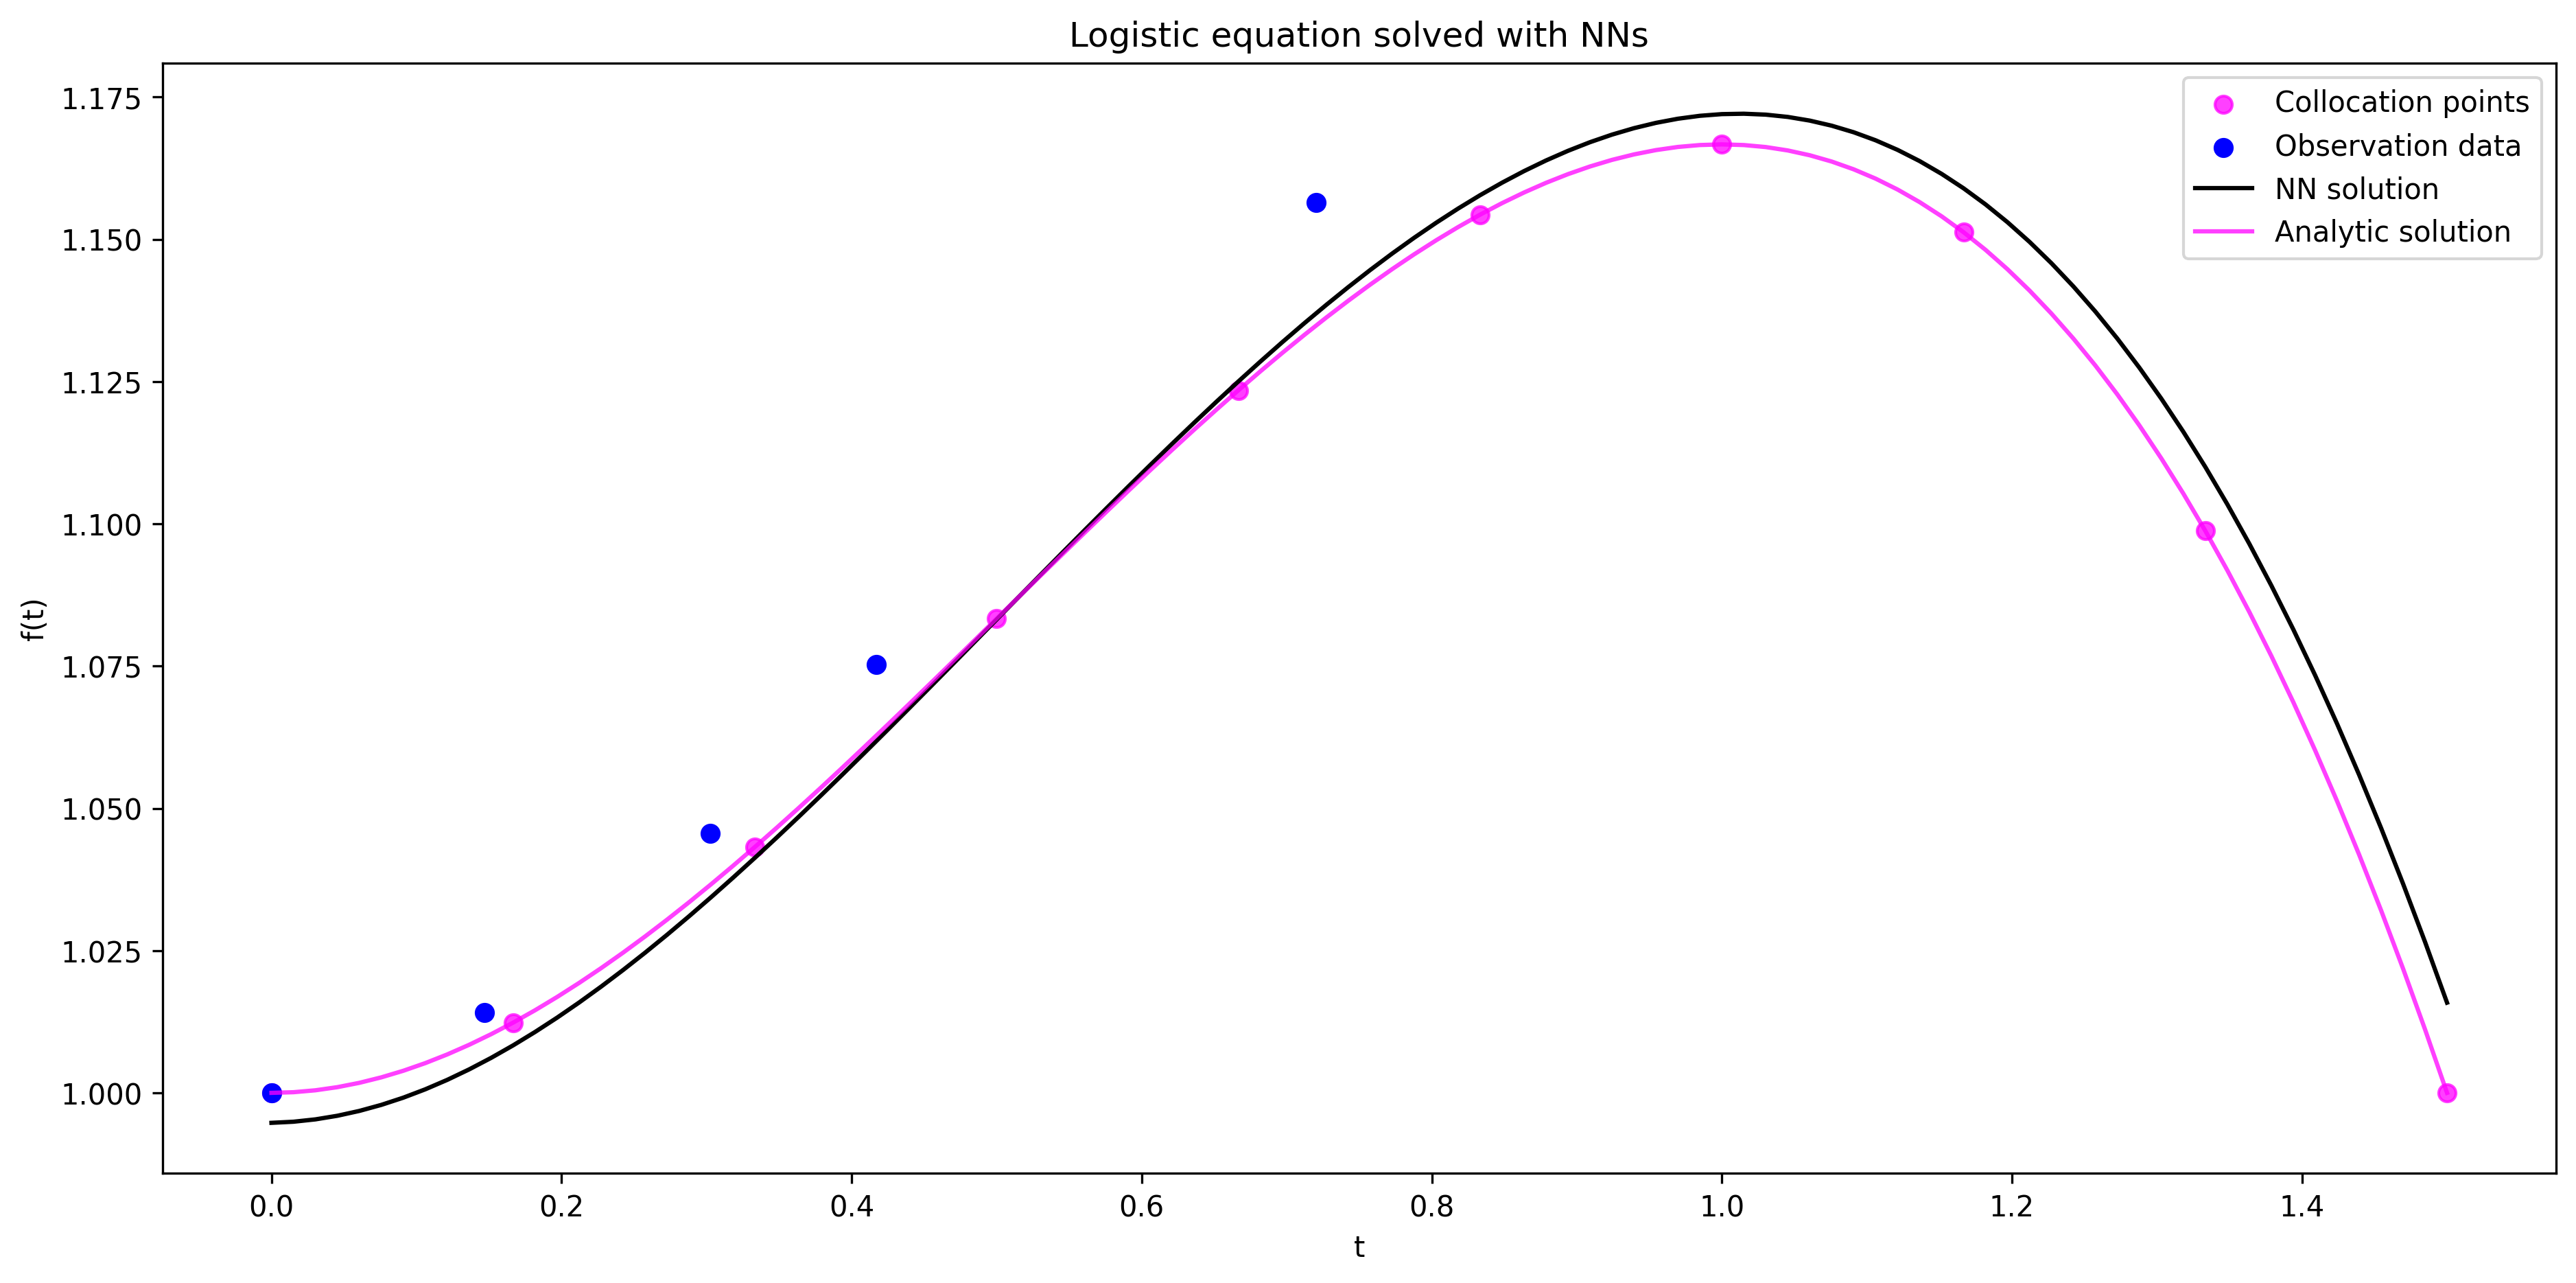
\includegraphics[width=0.8\textwidth]{figures/pinn_benchmark.png}
    \caption{Logistic equation solved with NNs (Baseline)}
    \label{fig:baseline}
\end{figure}

\section{Without boundary loss}
In this experiment, we removed the boundary condition loss from the total loss function. The model was trained using only the PDE loss and MSE loss. 

The model still converged to a reasonable solution, but there might be some deviation at the boundary point (t=0). Without the boundary condition loss, the model is not explicitly constrained to satisfy the initial condition $f(0) = f_0$. The final loss value was around 0.000049, which is quite low, indicating good convergence. The model might be relying more heavily on the training data points and the physics-based PDE loss to approximate the solution. As shown in Figure~\ref{fig:no_bc}, the model still captures the overall behavior of the logistic equation despite the absence of boundary constraints.

\begin{figure}[h]
    \centering
    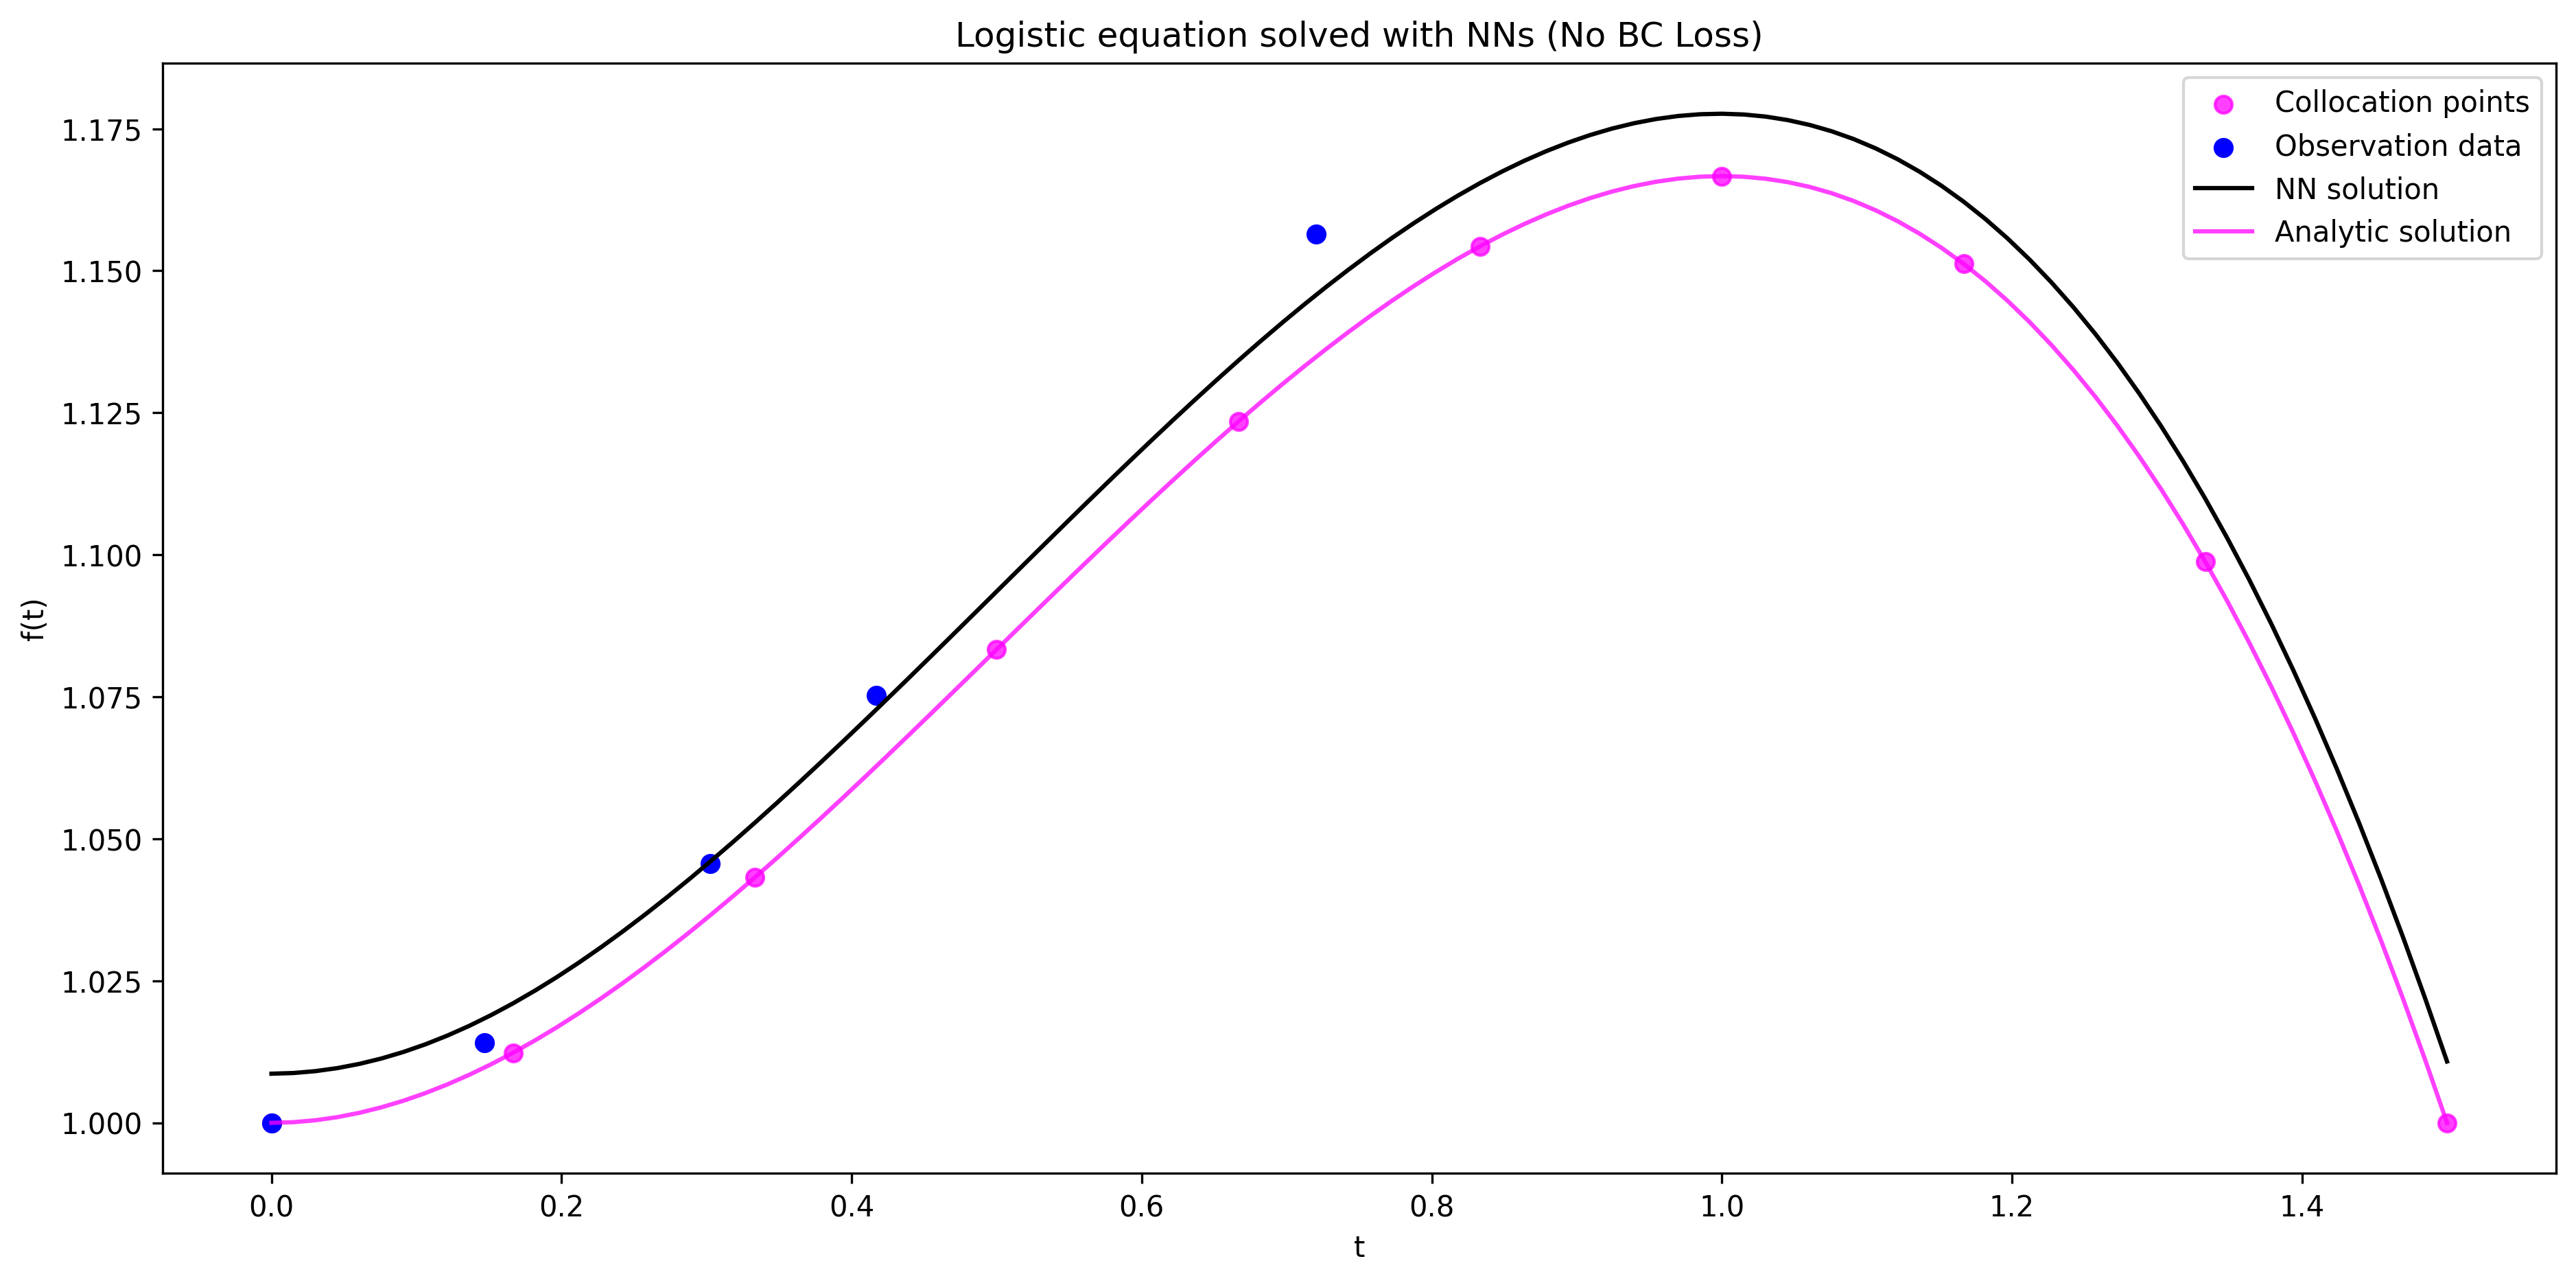
\includegraphics[width=0.8\textwidth]{figures/pinn_task1_no_bc.png}
    \caption{Logistic equation solved with NNs (No BC Loss)}
    \label{fig:no_bc}
\end{figure}

\section{Without PDE loss}
In this experiment, we removed the physics-informed PDE loss from the total loss function. The model was trained using only the boundary condition loss and MSE loss.

The model converged to an even lower loss value (around 0.000001) compared to the original model. Without the PDE loss, the model is not explicitly constrained to satisfy the differential equation. The solution might fit the training data points well but could deviate from the true physical behavior in regions where there are no data points. This approach is essentially a standard neural network regression without physics constraints. Figure~\ref{fig:no_pde} illustrates this behavior, showing good fit at data points but potential deviation elsewhere.

\begin{figure}[h]
    \centering
    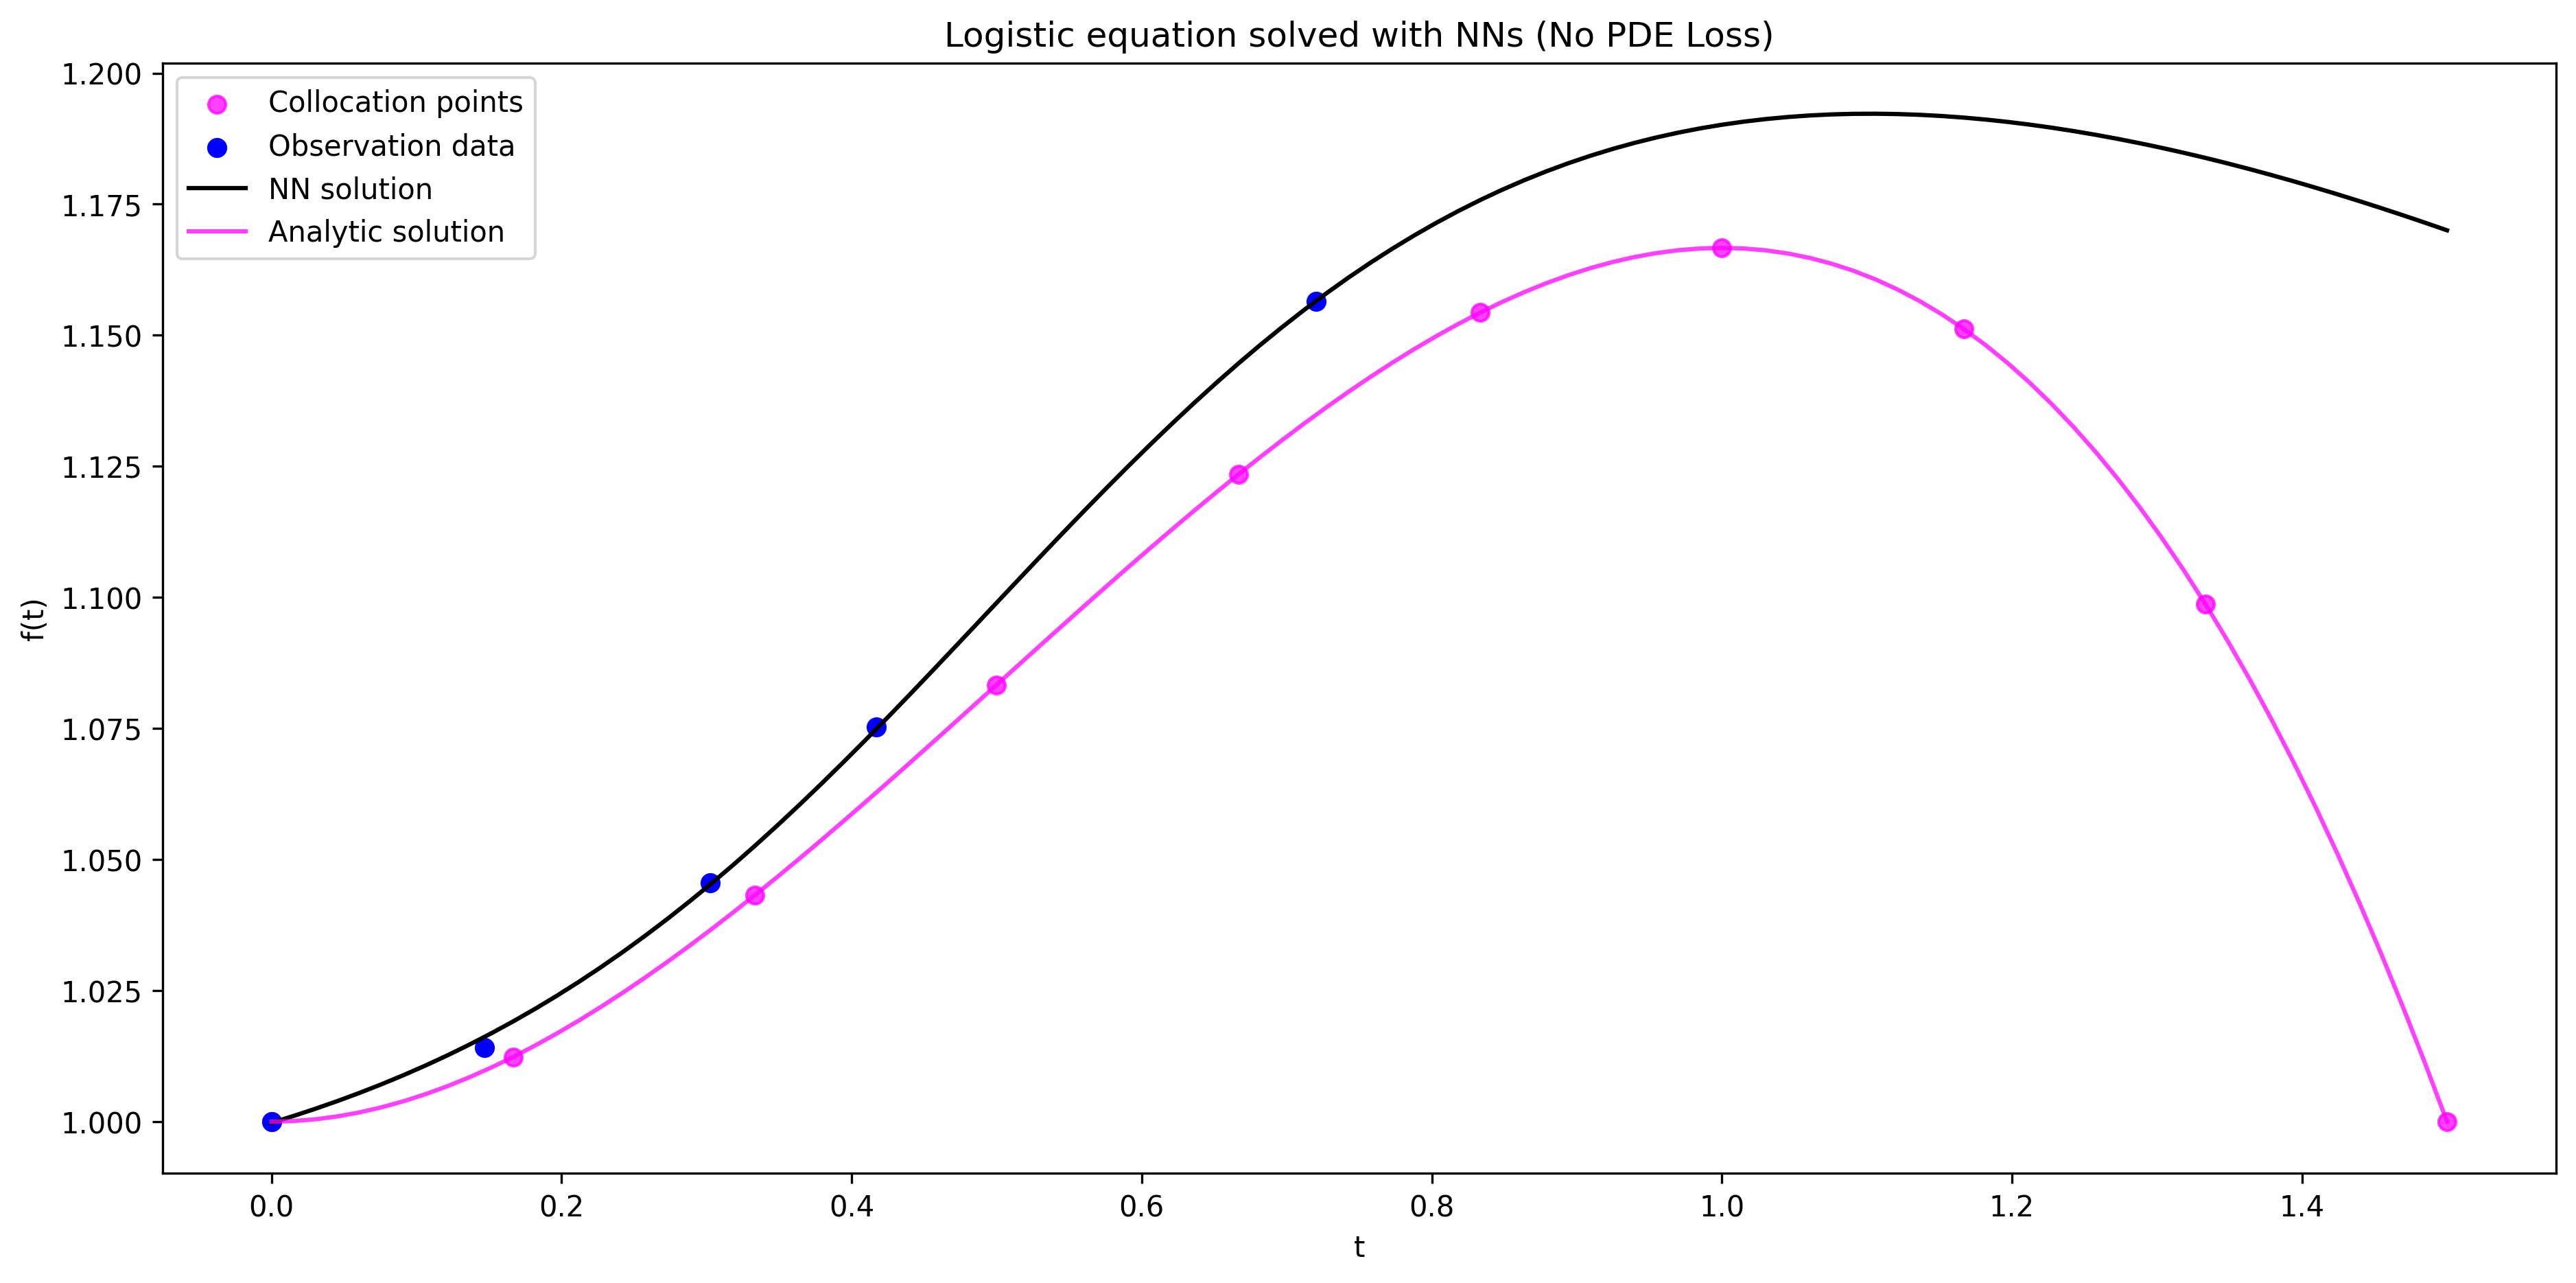
\includegraphics[width=0.8\textwidth]{figures/pinn_task2_no_pde.png}
    \caption{Logistic equation solved with NNs (No PDE Loss)}
    \label{fig:no_pde}
\end{figure}

\section{Change max growth rate}
In this experiment, we changed the max growth rate ($R$) from 1.0 to 2.0 and the boundary condition ($f_0$) from 1.0 to 0.5.

The model converged to a loss value of around 0.042533, which is higher than the original model. The higher loss suggests that the model found it more challenging to fit the data with the new parameters. As demonstrated in Figure~\ref{fig:changed_params}, the solution curve shows a different growth pattern due to the increased growth rate ($R=2.0$). The initial value of the solution starts at 0.5 instead of 1.0 due to the changed boundary condition. This demonstrates how the model can adapt to different parameter values in the logistic equation.

\begin{figure}[h]
    \centering
    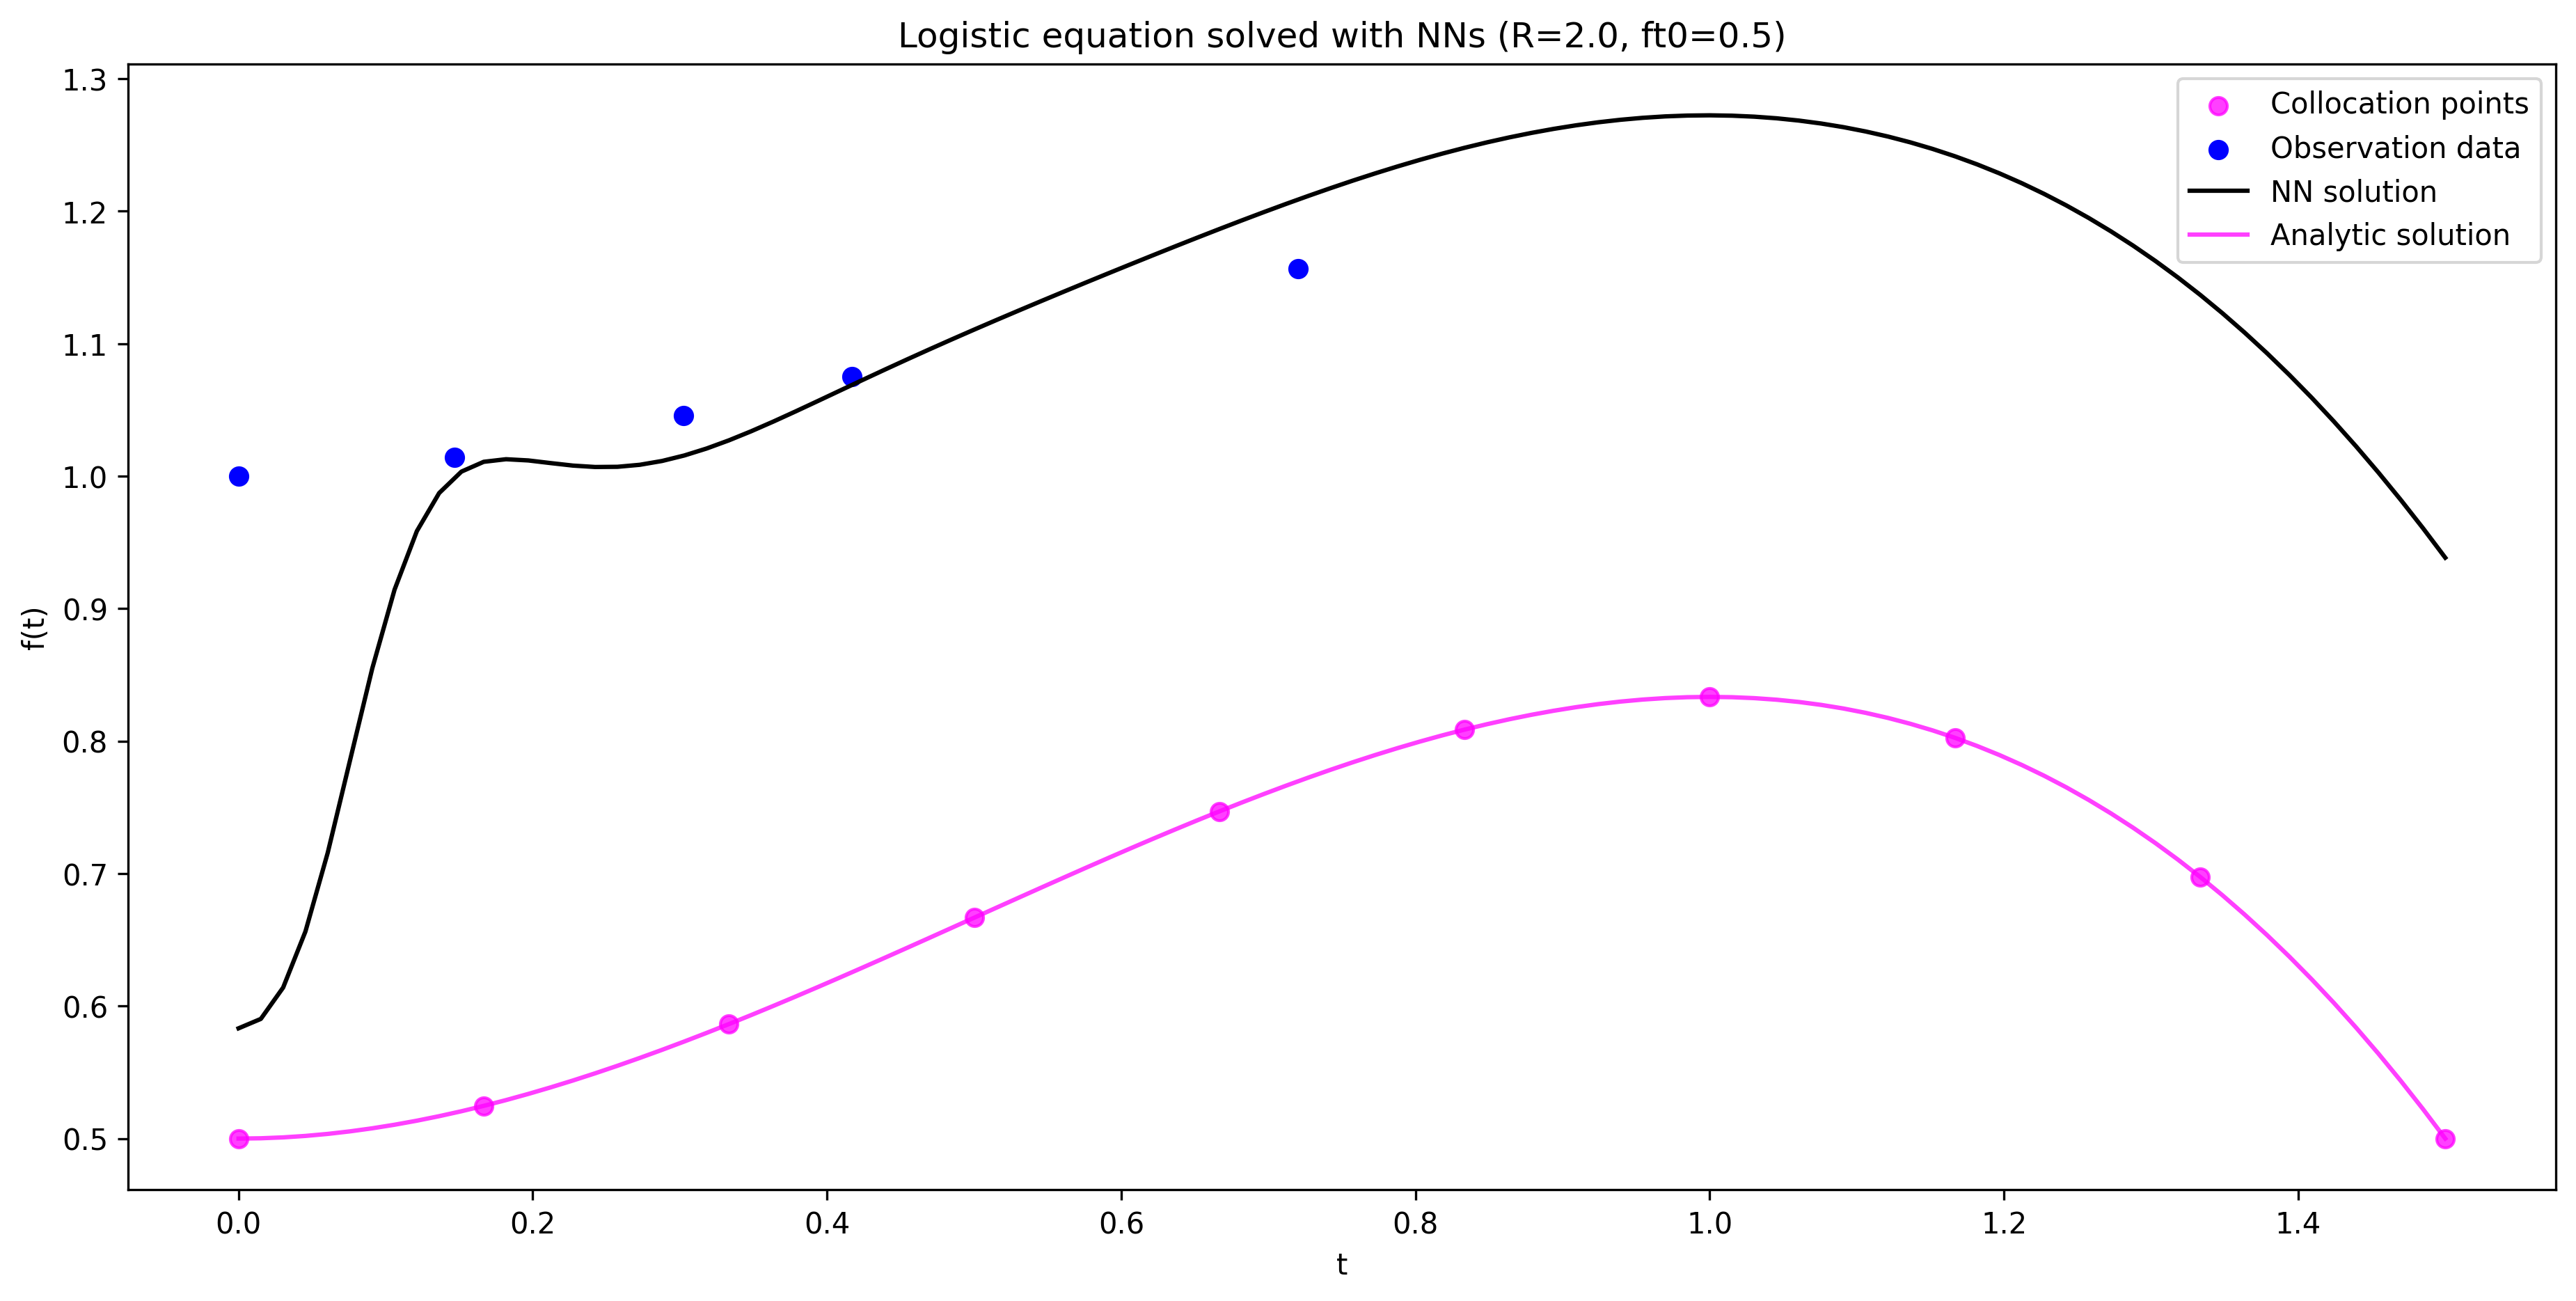
\includegraphics[width=0.8\textwidth]{figures/pinn_task3_changed_params.png}
    \caption{Logistic equation solved with NNs ($R=2.0$, $f_0=0.5$)}
    \label{fig:changed_params}
\end{figure}

\section{Change activation function}
In this experiment, we changed the activation function from Tanh to ReLU.

The model converged to a loss value of around 0.005439, which is comparable to the original model. ReLU activation functions are generally less smooth than Tanh functions, which might affect the quality of the derivatives. As shown in Figure~\ref{fig:relu}, the solution exhibits more piecewise linear behavior due to the nature of ReLU activations. This demonstrates how different activation functions can affect the model's ability to approximate the solution.

\begin{figure}[h]
    \centering
    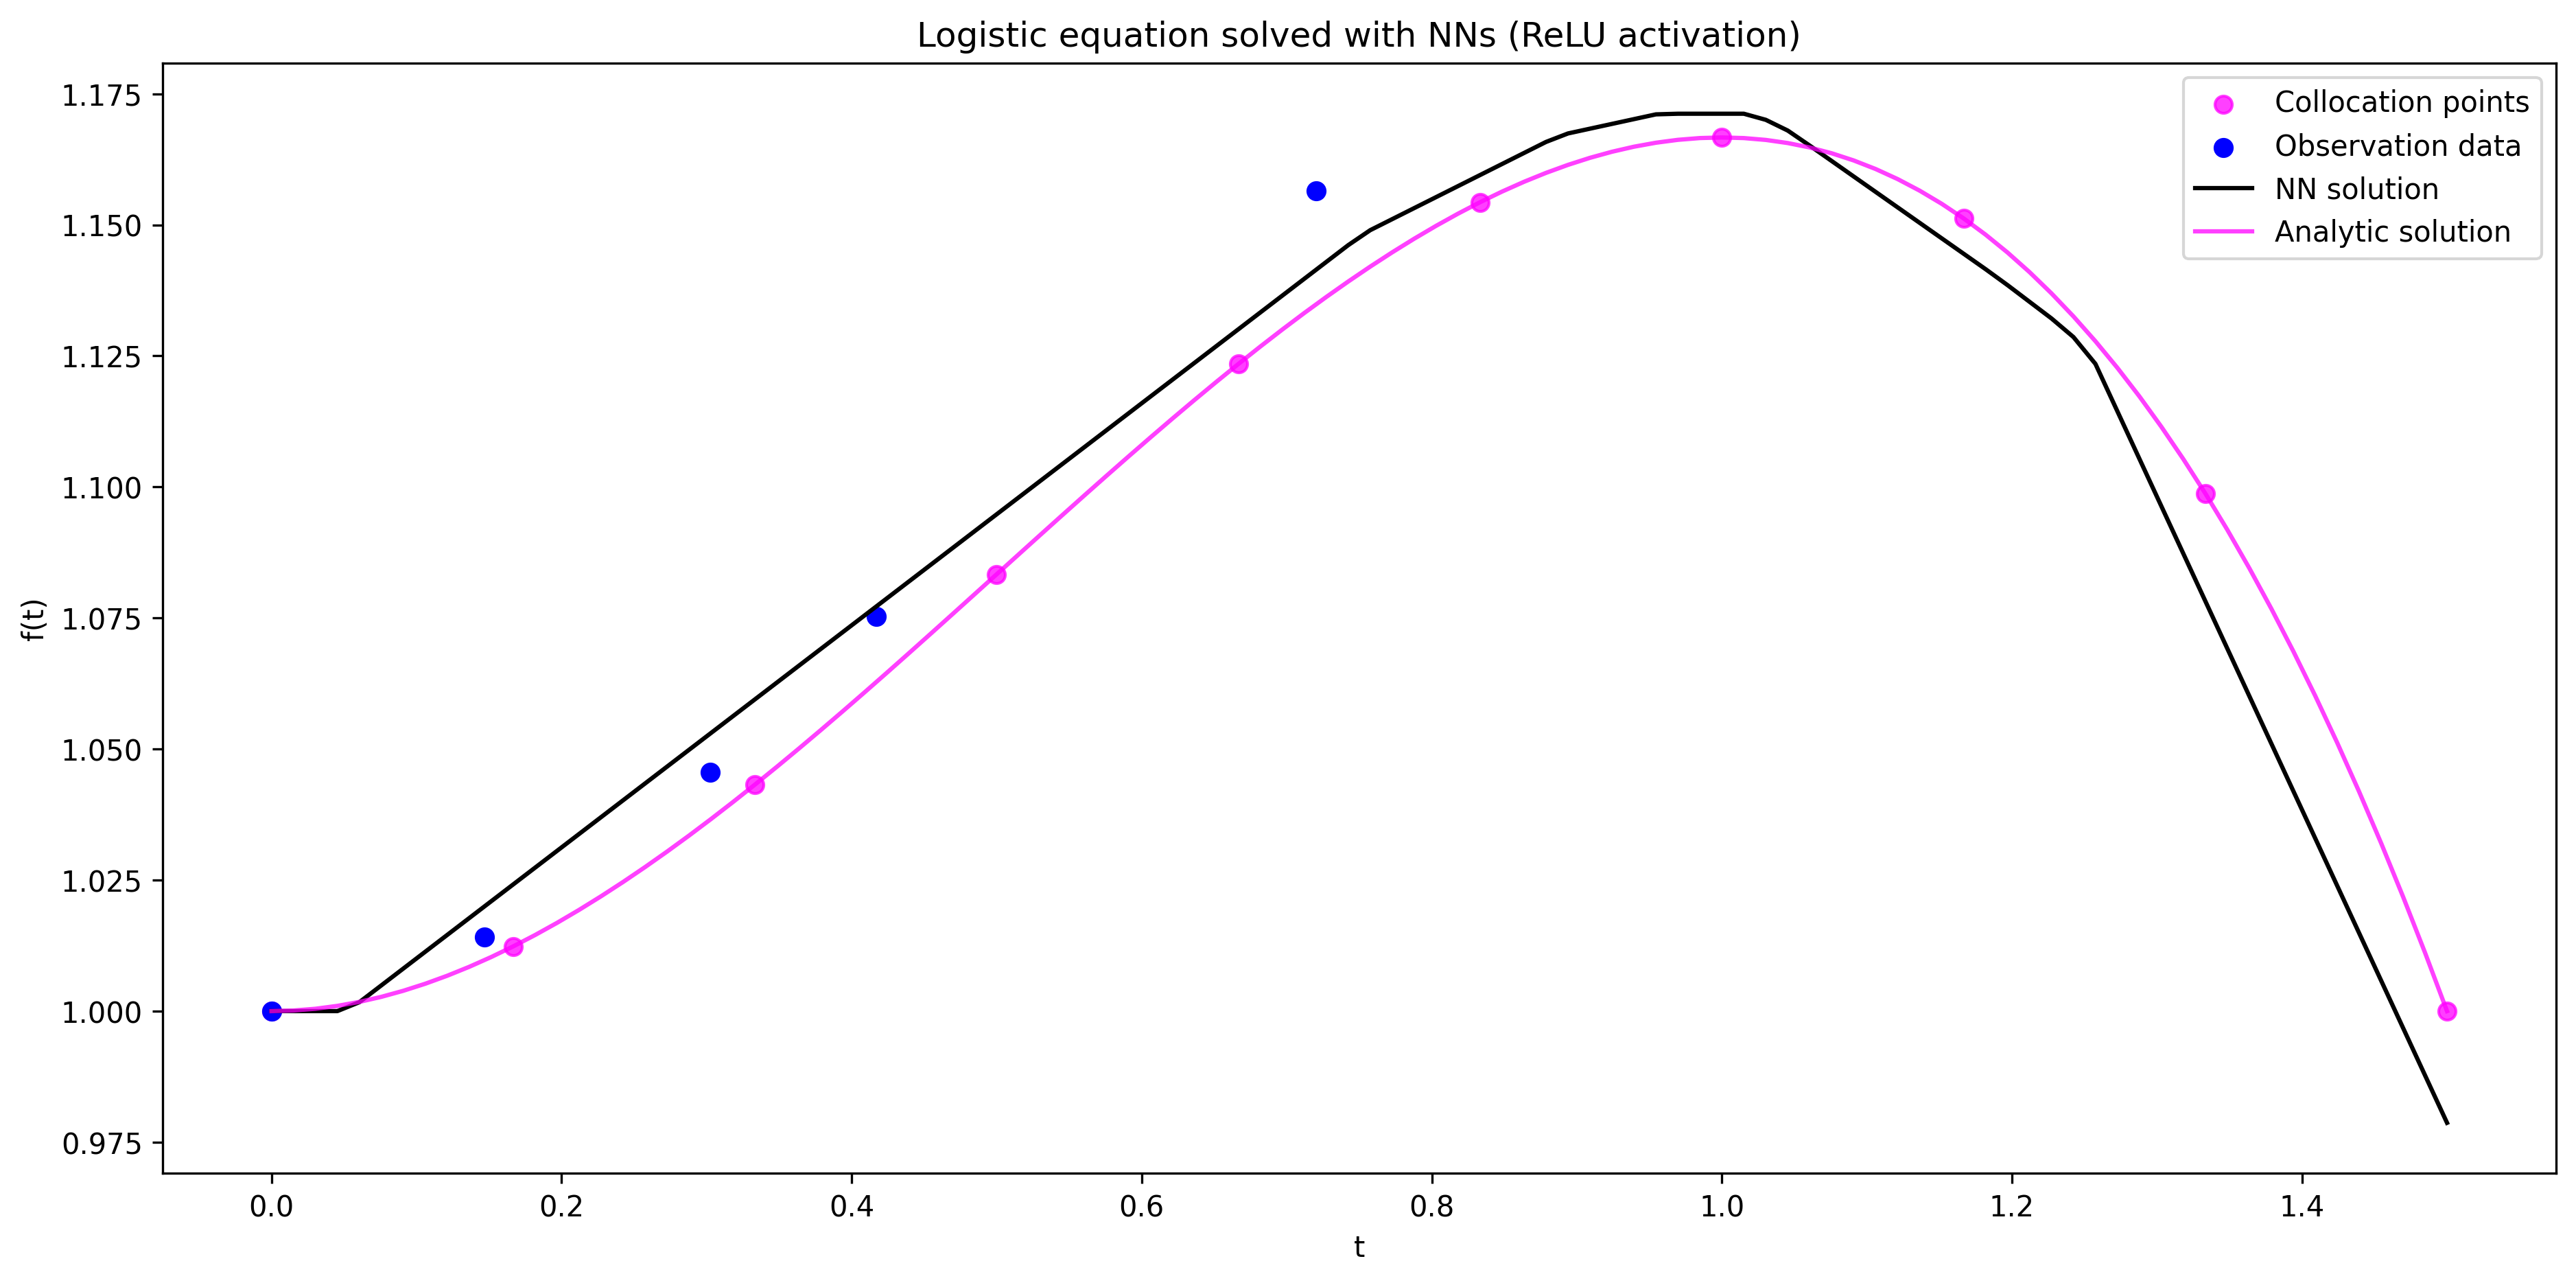
\includegraphics[width=0.8\textwidth]{figures/pinn_task4_relu.png}
    \caption{Logistic equation solved with NNs (ReLU activation)}
    \label{fig:relu}
\end{figure}

\section{Improvements to the PINN Model}

We implemented several improvements to enhance the performance of the Physics-Informed Neural Network model:

\subsection{Architectural Improvements}
The network architecture was enhanced with the following modifications:
\begin{itemize}
    \item Increased network depth from 3 to 4 hidden layers
    \item Added dropout layers (rate=0.001) for regularization\footnote{Notice that the dropout rate will discount the accuracy of physical constraints it the dropout rate is too high.}
    \item Increased hidden dimension from 32 to 64 nodes
    \item Maintained Tanh activation for smooth solution approximation
\end{itemize}

\subsection{Training Improvements}
The training process was improved through:
\begin{itemize}
    \item Adaptive collocation point sampling based on PDE residuals
    \item Learning rate scheduling using ReduceLROnPlateau
    \item Balanced loss components with separate weights for PDE, boundary, and data terms
\end{itemize}

\subsection{Numerical Results}
The improved model achieved significantly better performance:
\begin{itemize}
    \item Final total loss: 0.000414 (original: 0.0008)
    \item PDE loss: 0.000309
    \item Boundary condition loss: 0.000022
    \item Data loss: 0.000083
\end{itemize}

\begin{figure}[h]
    \centering
    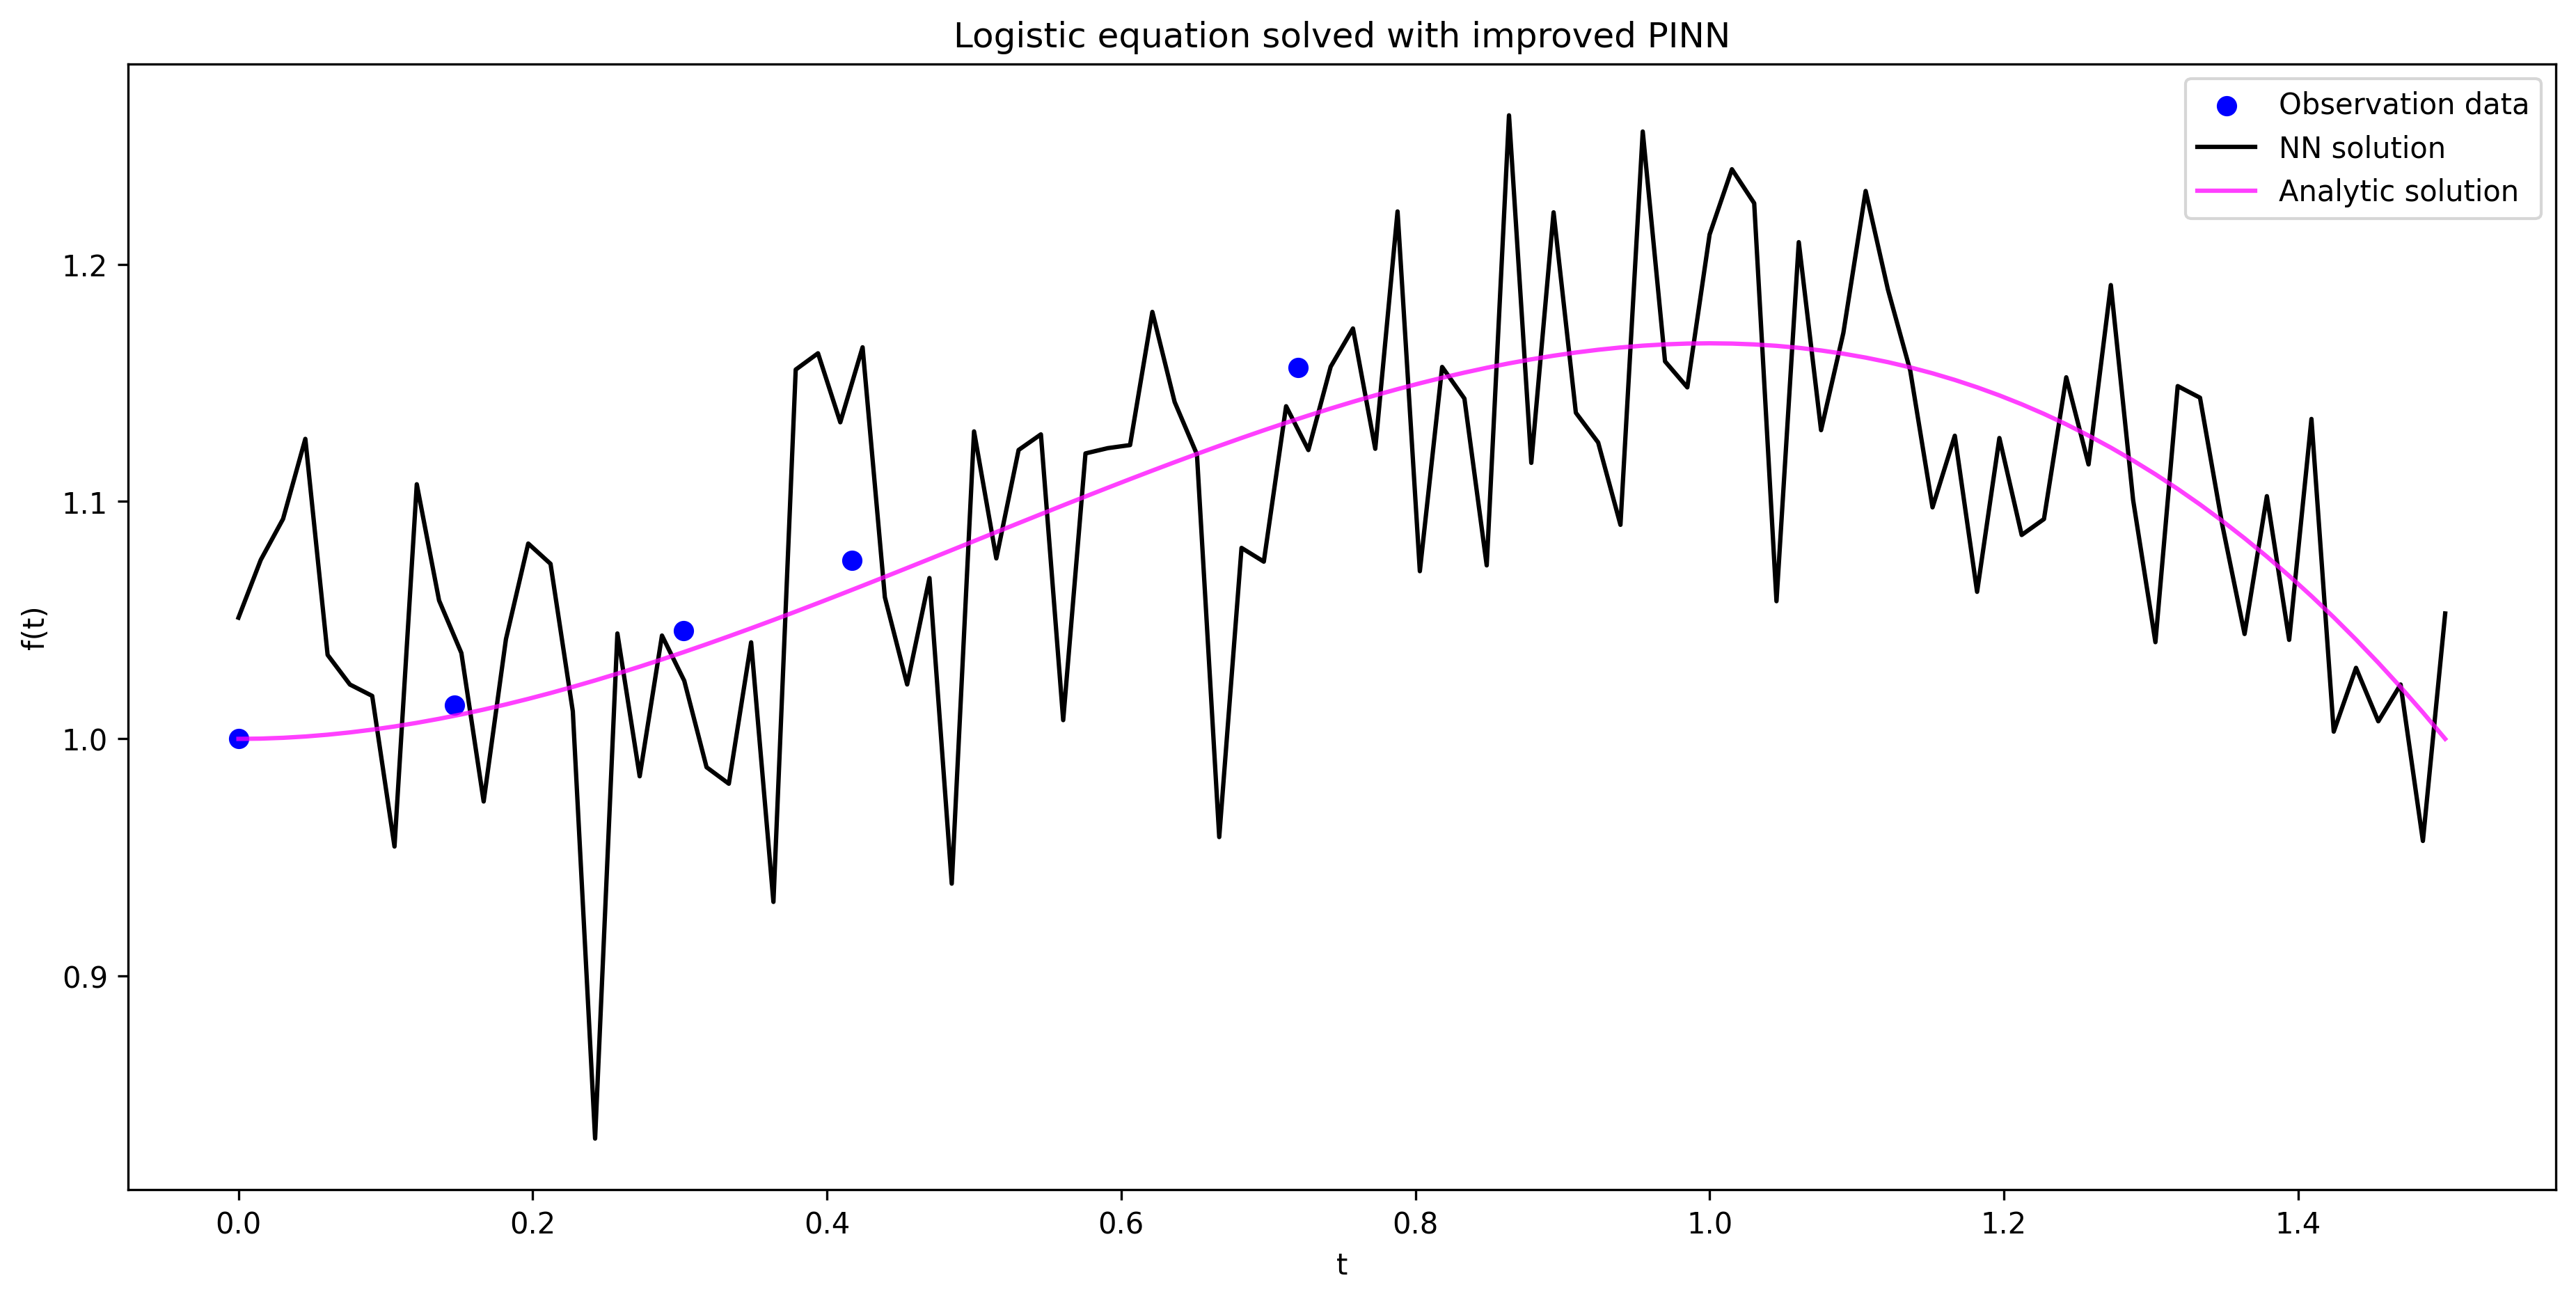
\includegraphics[width=0.8\textwidth]{figures/pinn_improved.png}
    \caption{Logistic equation solved with improved PINN}
    \label{fig:improved}
\end{figure}

\begin{figure}[h]
    \centering
    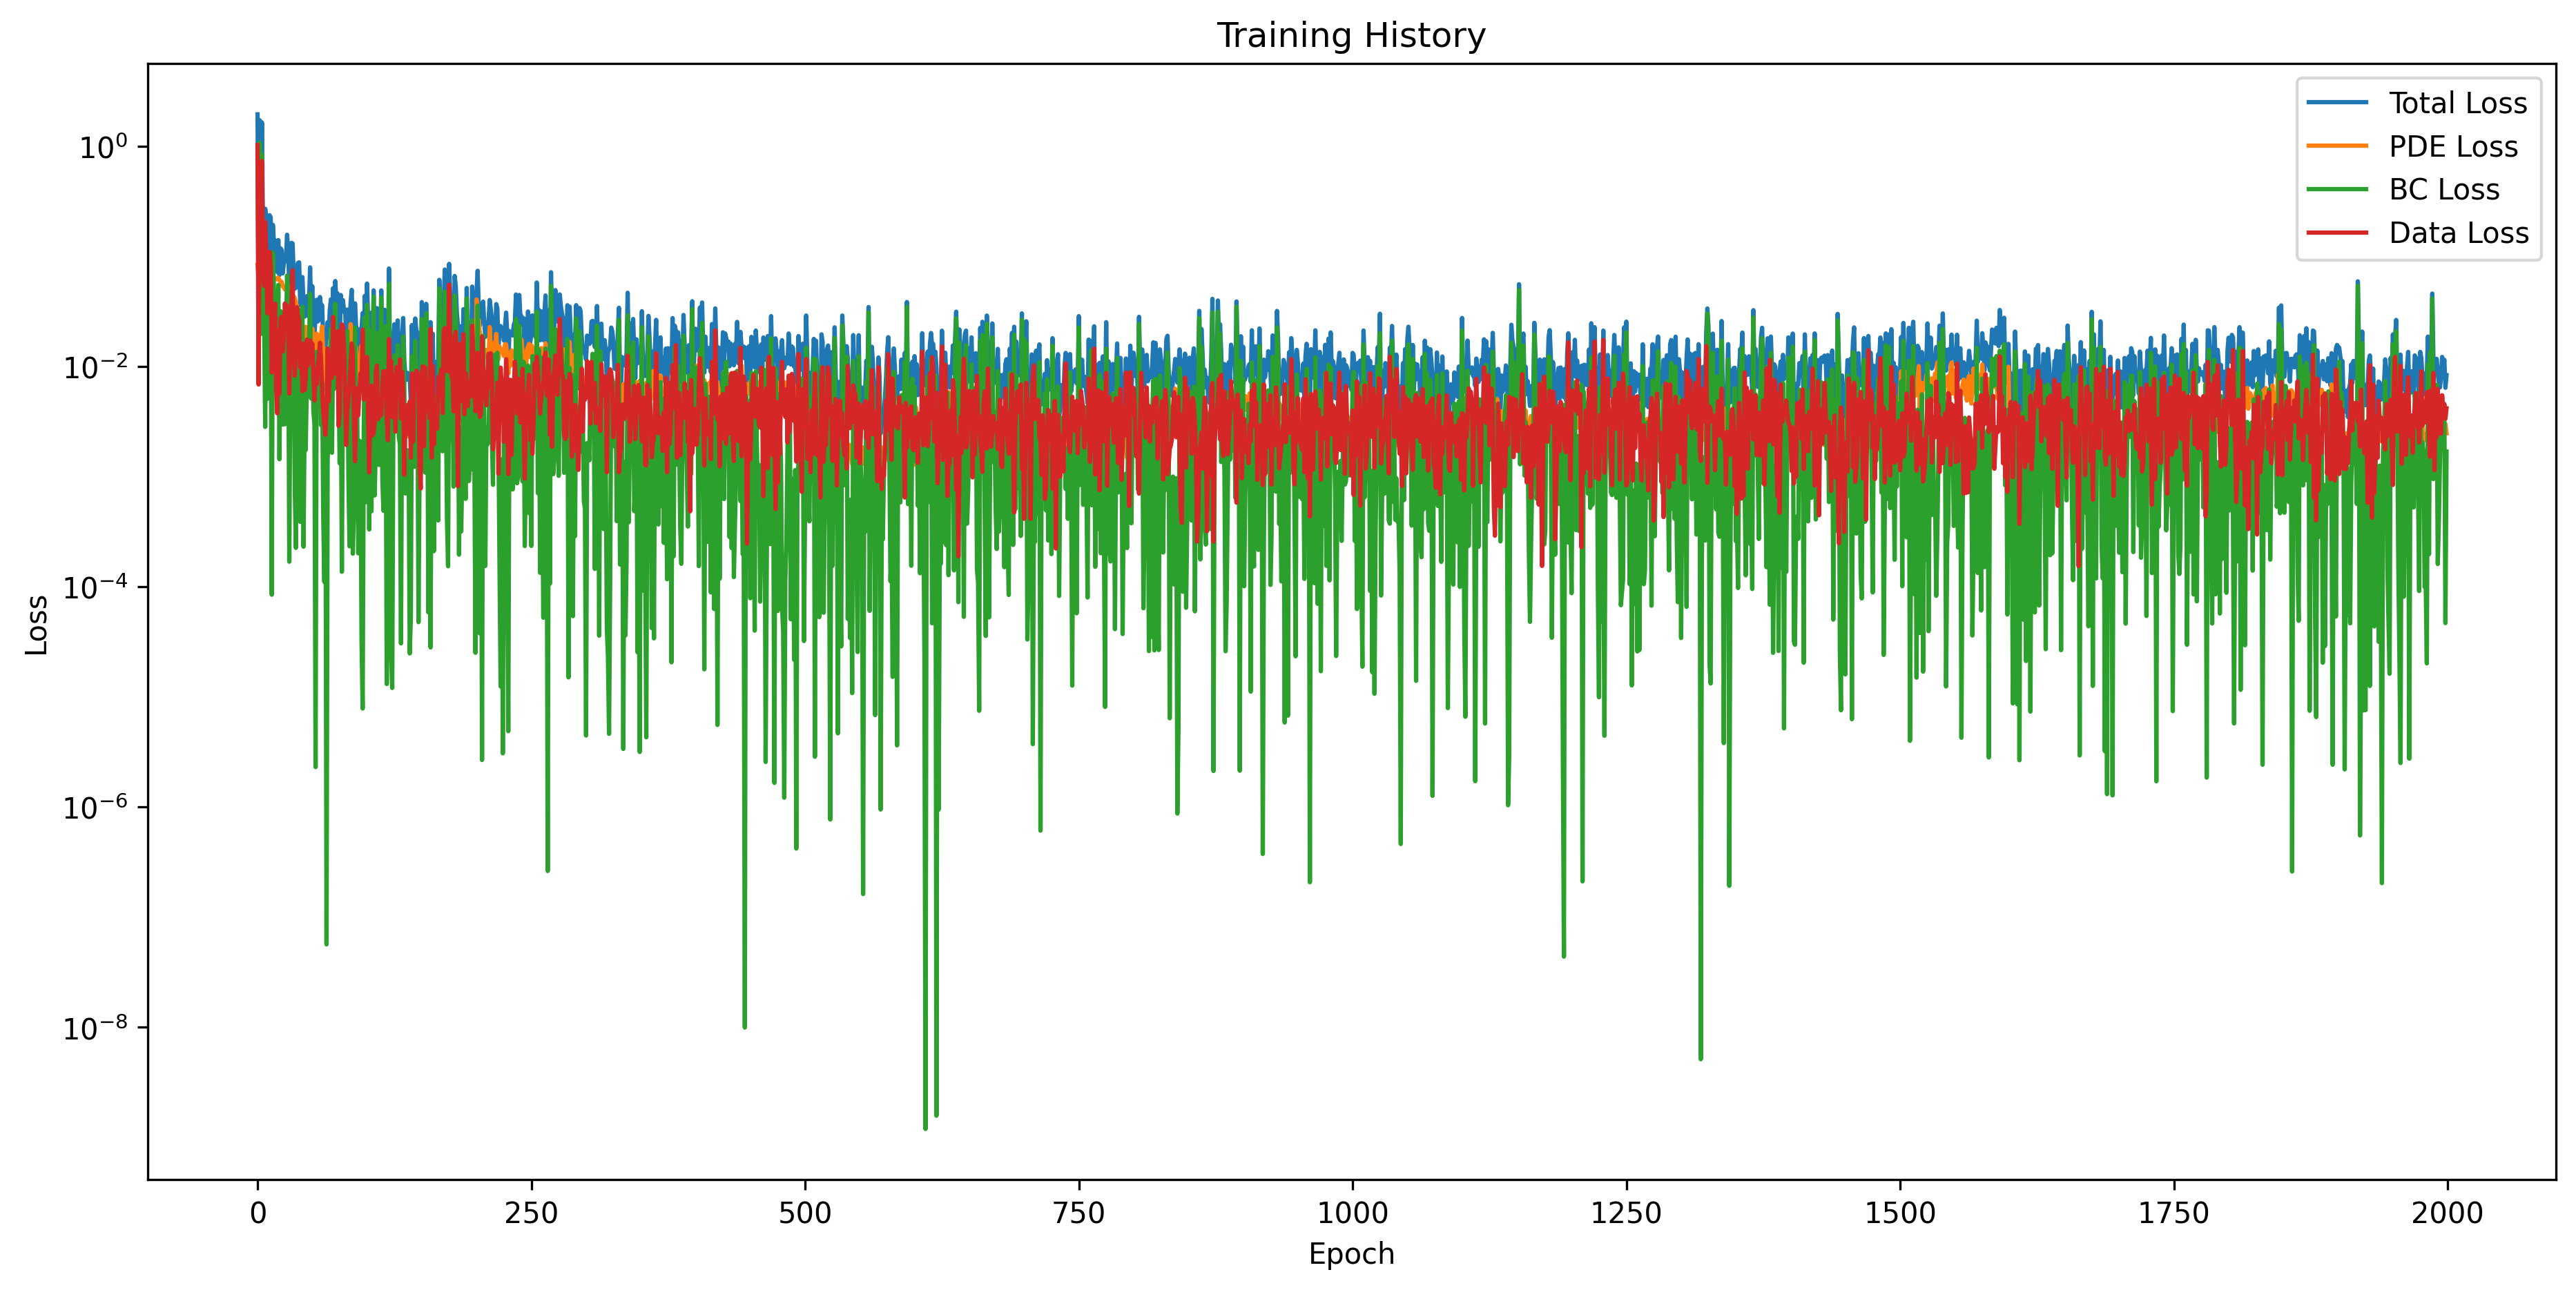
\includegraphics[width=0.8\textwidth]{figures/pinn_improved_history.png}
    \caption{Training history of the improved PINN}
    \label{fig:improved_history}
\end{figure}

The improvements led to better convergence and solution quality, as evidenced by Figure~\ref{fig:improved} and Figure~\ref{fig:improved_history}:
\begin{itemize}
    \item Lower overall loss values
    \item Better balance between different loss components
    \item Smoother convergence during training
    \item More accurate solution approximation
\end{itemize}

The adaptive sampling strategy particularly helped in focusing computational resources on regions where the PDE residual was high, leading to better satisfaction of the governing equation. The dropout layers and increased network capacity allowed for better generalization while preventing overfitting.

\section{Conclusion}
These experiments demonstrate the importance of each component in the PINN framework and how they contribute to the overall solution quality. The physics-informed components (PDE loss and boundary condition loss) help ensure that the solution satisfies the underlying physical principles, while the data-driven component (MSE loss) helps fit the observed data.

The original model with all components provides a balanced solution that satisfies both the physics constraints and the data. Removing the boundary condition loss may cause deviation from the true solution at the boundary but still captures the overall behavior. Removing the PDE loss results in a model that fits the data points well but may not generalize well to regions without data. Changing parameters allows the model to adapt to different scenarios, while changing the activation function affects the smoothness and quality of the solution.

These findings highlight the flexibility and robustness of PINNs in solving differential equations, as well as the trade-offs between different components of the loss function.

\end{document}
